

\chapter{Верификация окружения и архитектуры}

Номер ИСУ: 466625

Порт: 5430 + 25 = 5455

Префикс: manuk 

Выполнили 2 команды для просмотра версии и архитектуры. Вывод терминала представлен на рисунке \ref{first}.

\begin{Verbatim}
docker version --format "Client: {{.Client.Version}}, Server: {{.Server.Version}}"
docker info --format "{{.OSType}}/{{.Architecture}}"
\end{Verbatim}

 \begin{figure}[H]
\centerline{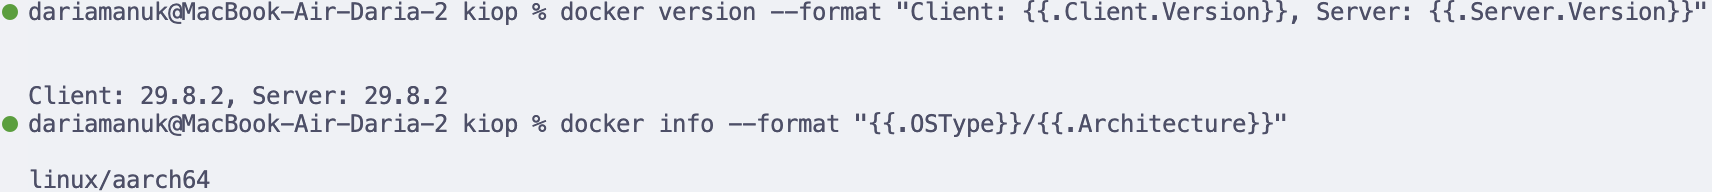
\includegraphics[width= 0.70\textwidth]{pic/1.png}}
\caption{Терминальный вывод}
\label{first}
\end{figure}


Далее провели проверку количества образов и контейнеров существующих до работы. (рисунок \ref{sec})

\begin{Verbatim}
docker system df --format "table {{.Type}}\t{{.TotalCount}}\t{{.Active}}\t{{.Size}}"
\end{Verbatim}

\begin{figure}[H]
\centerline{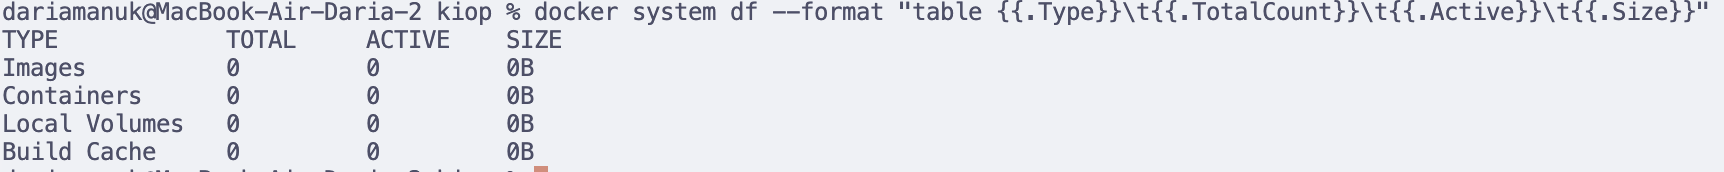
\includegraphics[width= 0.70\textwidth]{pic/2.png}}
\caption{Терминальный вывод}
\label{sec}
\end{figure}

Вопросы:
\begin{enumerate}
    \item docker version без запуска самого докера выдает ошибку (\ref{version})
    \item docker system prune удаляет все остановленные контейнеры, а также неиспользуемые сети, dangling-образы и dangling build cache.
\end{enumerate}


\begin{figure}[H]
\centerline{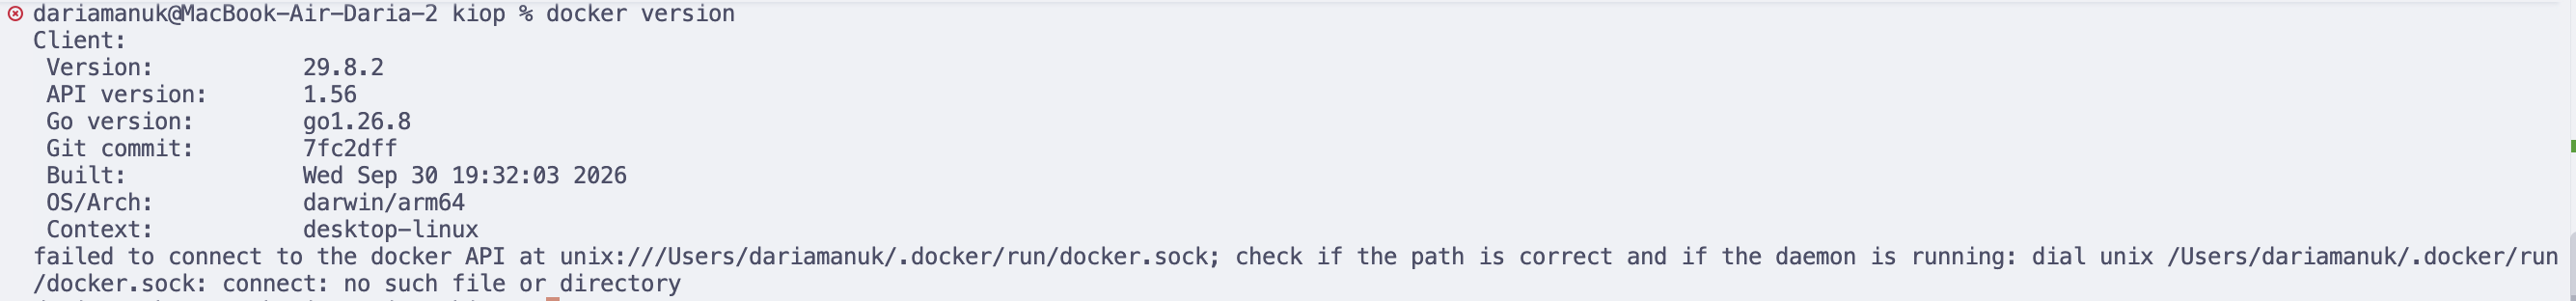
\includegraphics[width= 0.70\textwidth]{pic/version.png}}
\caption{Терминальный вывод}
\label{version}
\end{figure}

\chapter{Первые шаги: «игрушечные» образы}

Запускаем классический пример (рисунок \ref{hello}). Как видно из первых строчек, образ запускается из library/hello-world:latest. Выполняется процесс /hello.

\begin{Verbatim}
docker run --rm hello-world
docker image inspect hello-world --format 'Entrypoint: {{.Config.Entrypoint}}  Cmd: {{.Config.Cmd}}'
\end{Verbatim}

\begin{figure}[H]
\centerline{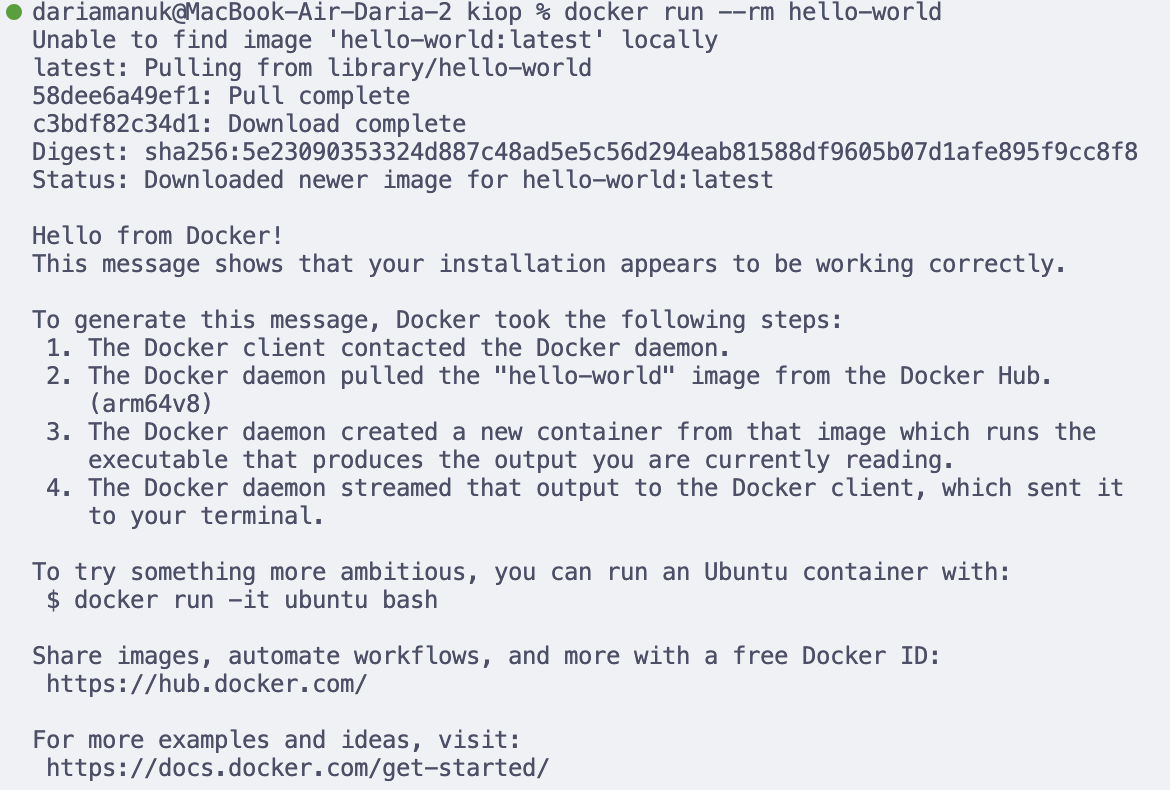
\includegraphics[width= 0.70\textwidth]{pic/hello.png}}
\caption{Терминальный вывод}
\label{hello}
\end{figure}

Запускаем минимальный образ. (рисунок \ref{alpine})

\begin{Verbatim}
docker run --rm alpine:3.18 cat /etc/os-release
docker images alpine:3.18 --format "{{.Size}}"
\end{Verbatim}

\begin{figure}[H]
\centerline{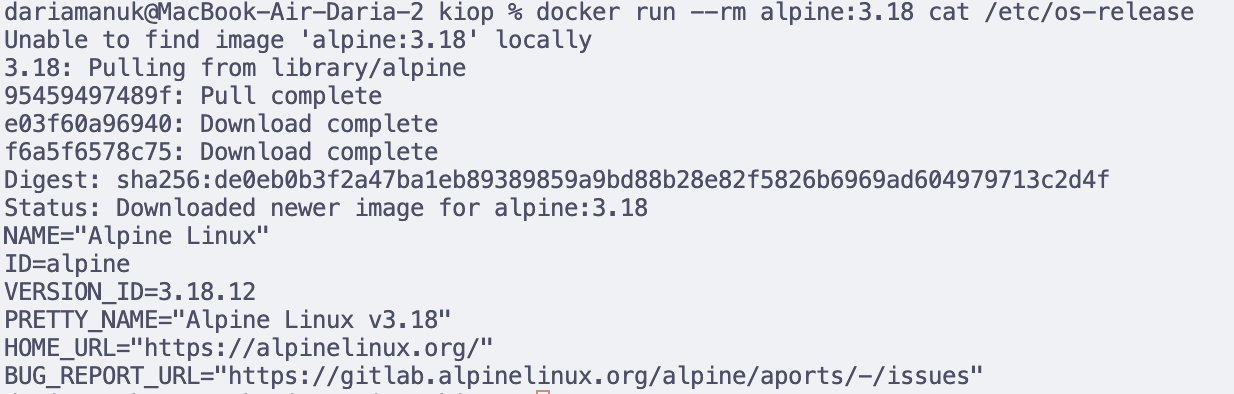
\includegraphics[width= 0.70\textwidth]{pic/alpine.png}}
\caption{Терминальный вывод}
\label{alpine}
\end{figure}

PRETTY\_NAME="Alpine Linux v3.18" , 11.8MB

Пробуем запустить новый контейнер с удерживанием процесса. (рисунок \ref{filter})

\begin{Verbatim}
docker run -d --name manuk-alpine-1 alpine:3.18 sleep 300
docker run -d --name manuk-alpine-2 alpine:3.18 sh -c "echo 'Hello from $(hostname)' && sleep 300"
docker ps --filter "name=manuk-alpine"
\end{Verbatim}

\begin{figure}[H]
\centerline{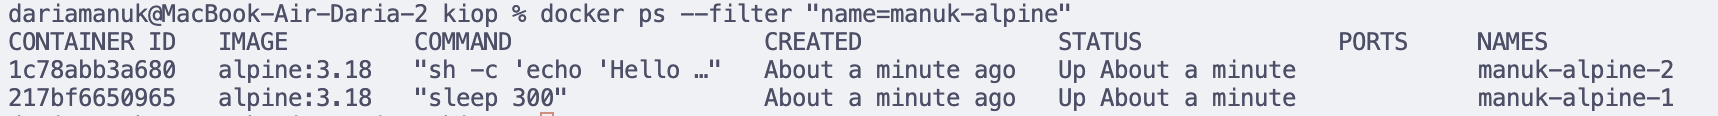
\includegraphics[width= 0.70\textwidth]{pic/filter.png}}
\caption{Терминальный вывод}
\label{filter}
\end{figure}

Вопросы:
\begin{enumerate}
    \item Запускается программа, и контейнер завершает работу сразу после ее выполнения, sleep 300 ждет конца таймера или до завершения процесса.
    \item --rm сразу удаляет контейнер после завершения работы, без него коннтейнер будет в состоянии exited. Для удаления можно использовать разные команды docker rm name/id или docker container prune.
\end{enumerate}

\chapter{Жизненный цикл контейнера}

Проследили статусы контейнеров на каждом этапе его жизненного цикла (рисунок \ref{status})
\begin{Verbatim}
docker create --name manuk-nginx nginx:alpine

docker start manuk-nginx

docker stop manuk-nginx

docker restart manuk-nginx

docker kill manuk-nginx

docker rm manuk-nginx

docker ps -a --filter "name=manuk-nginx" --format "table {{.Names}}\t{{.Status}}\t{{.CreatedAt}}"
\end{Verbatim}

\begin{figure}[H]
\centerline{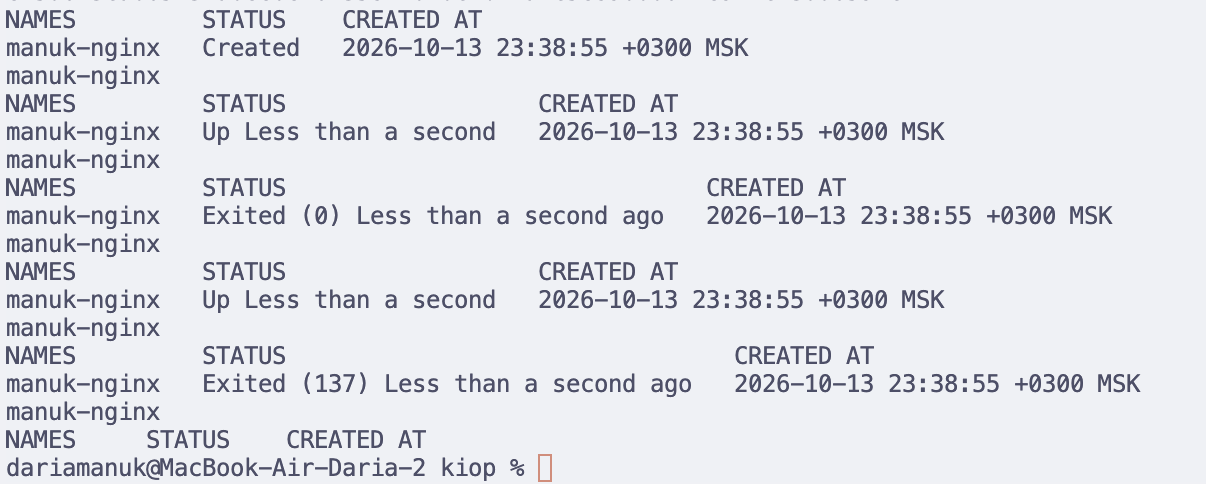
\includegraphics[width= 0.70\textwidth]{pic/status.png}}
\caption{Терминальный вывод}
\label{status}
\end{figure}

SIGTERM - graceful shutdown, процесс дается время на корректное завершение и очистку занятых ресурсов, в отличие от SIGKILL, и если процесс записи данных не завершился, то будут удалены при kill. 

Вопросы:
\begin{enumerate}
    \item Ошибка вызова команды представлена на рисунке \ref{error}
    \item Нужен флаг -f -force или сначала остановить его.
\end{enumerate}

\begin{figure}[H]
\centerline{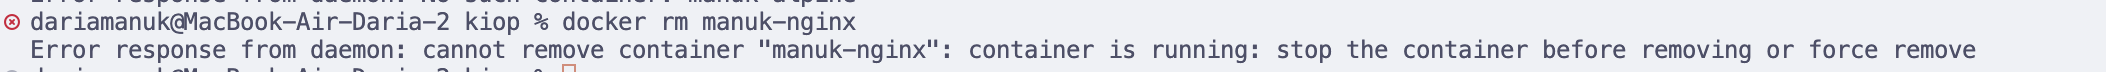
\includegraphics[width= 0.70\textwidth]{pic/error.png}}
\caption{Терминальный вывод}
\label{error}
\end{figure}

\chapter{Диагностика реального сервиса}

После установки образа не выдается ошибка из-за -d, но в диагностике видно. (рисунок \ref{d})

\begin{Verbatim}
docker run -d \
  --name manuk-pg-broken \
  -p 5455:5432 \
  postgres:15

docker ps -a --filter "name=manuk-pg"

docker logs --timestamps manuk-pg-broken 2>&1 | tail -20

docker inspect manuk-pg-broken --format='{{.State.ExitCode}}'

\end{Verbatim}

\begin{figure}[H]
\centerline{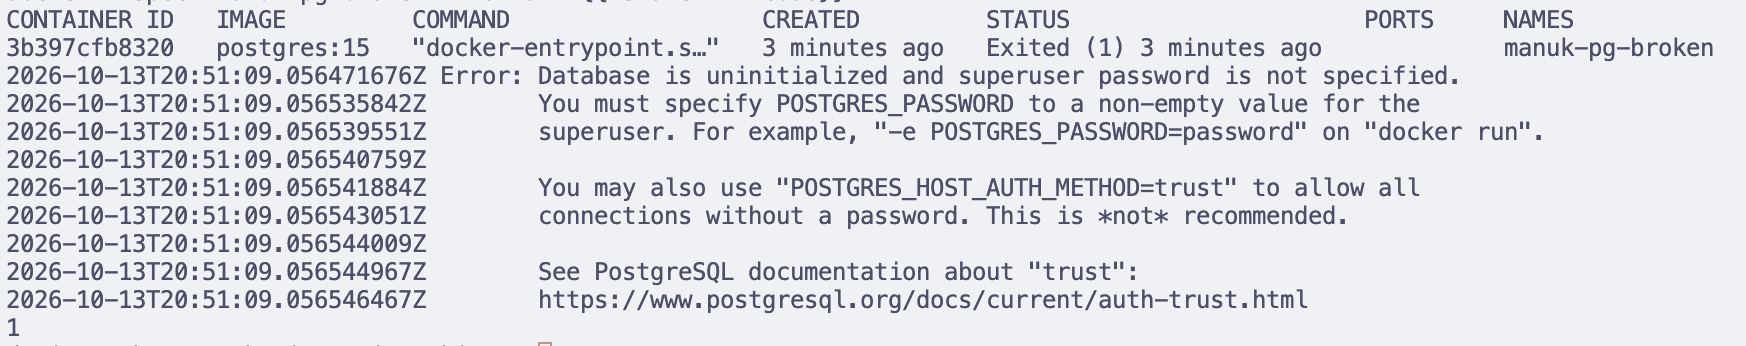
\includegraphics[width= 0.70\textwidth]{pic/d.png}}
\caption{Диагностика}
\label{d}
\end{figure}

Исправляем ошибку.

\begin{Verbatim}
docker run -d \
  --name manuk-pg-fixed \
  -e POSTGRES_PASSWORD=Pass_5455 \
  -e POSTGRES_USER=user_466625 \
  -p 5455:5432 \
  postgres:15

sleep 15

docker exec manuk-pg-fixed psql -U user_466625 -c "SELECT version();"
\end{Verbatim}

Финальный артефакт представлен на рисунке \ref{final}.

\begin{Verbatim}
echo "=== Практика №1: $(date '+%Y-%m-%d %H:%M:%S') ===" && \
echo "Студент: $(whoami)@$(hostname)" && \
docker ps --filter "name=<фамилия>-pg-fixed" --format "table {{.Names}}\t{{.Status}}\t{{.Ports}}"
\end{Verbatim}

\begin{figure}[H]
\centerline{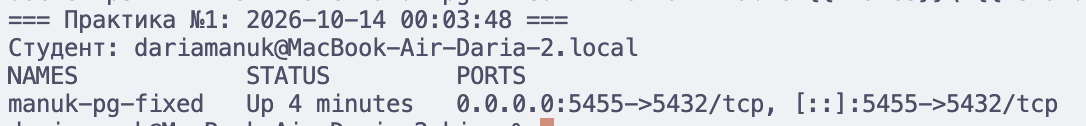
\includegraphics[width= 0.70\textwidth]{pic/final.png}}
\caption{Финальный артефакт}
\label{final}
\end{figure}
